\documentclass[border=10pt]{standalone}
\usepackage{tikz}

\begin{document}
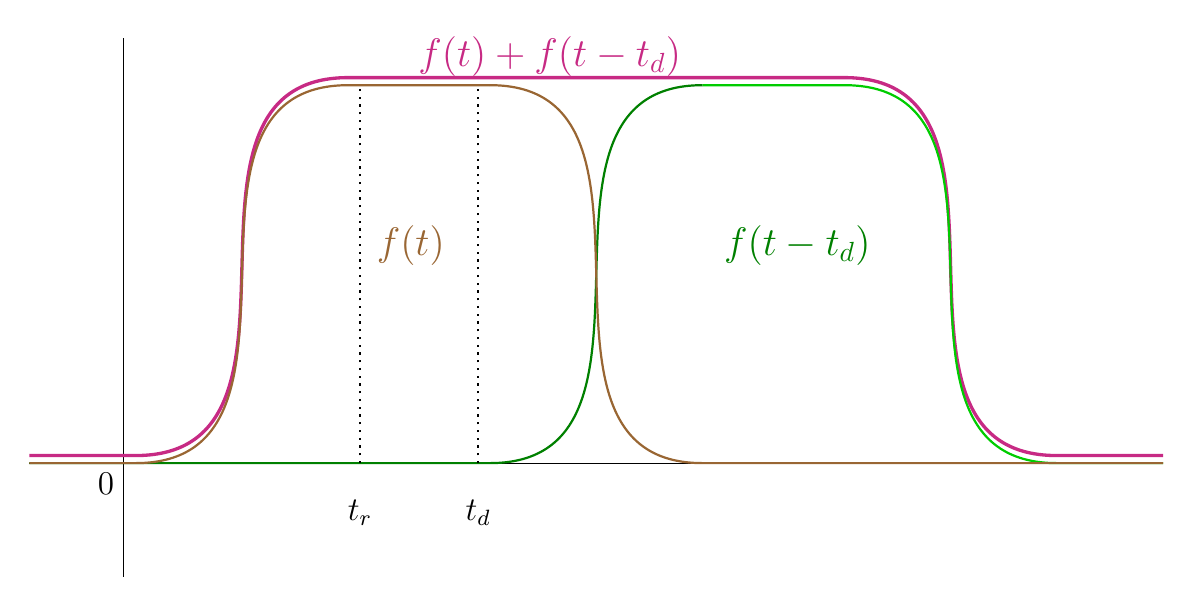
\begin{tikzpicture}[xscale=1.5, yscale=1.2]

  % Axes based on the images
  \draw (0,-1.2) -- (0,4.5);
  \draw (-0.8,0) -- (8.8,0);

  % Ticks
  \node[below left, font=\large] at (0,0) {0};
  % \foreach \x in {0,1,2,3,4,5,6,7,8} {
  %     % \draw (\x,0) -- (\x,-0.05);
  %     % \node[below left, font=\scriptsize] at (\x,0) {\x};
  %   }
  % \foreach \y in {-1,1,2,3,4} {
  %     % \draw (0,\y) -- (-0.05,\y);
  %     % \node[left, font=\scriptsize] at (-0.05,\y) {\y};
  %   }

  % Base Waveforms
  % Magenta curve (main envelope) - slightly lifted
  \draw[very thick, color=magenta!80!black] (-0.8,0.08) -- (0.1,0.08) to[out=0,in=180] (1.9,4.08) -- (6.1,4.08)
  to[out=0,in=180] (7.9,0.08) -- (8.8,0.08);
  \node[left, color=magenta!80!black, font=\Large] at (4.8, 4.3) {$f(t)+f(t-t_d)$};

  % Green curve (rising edge crossover)
  \draw[thick, color=green!50!black] (-0.8,0) -- (3.1,0) to[out=0,in=180] (4.9,4);
  \draw[thick, color=green!80!black] (4.9,4.00) -- (6.1,4.00) to[out=0,in=180] (7.9,0.00) -- (8.8,0.00);
  % Label for the green curve
  \node[right, color=green!50!black, font=\Large] at (5.0, 2.3) {$f(t-t_d)$};

  % Brown curve (falling edge crossover)
  \draw[thick, color=brown!80!black] (3.1,4) to[out=0,in=180] (4.9,0) -- (8.8,0);
  \draw[thick, color=brown!80!black] (-0.8,0.00) -- (0.1,0.00) to[out=0,in=180] (1.9,4.00) -- (3.1,4.00);
  % Label for the brown curve
  \node[left, color=brown!80!black, font=\Large] at (2.8, 2.3) {$f(t)$};

  % Dotted line additions
  \draw[dotted, thick] (2,0) -- (2,4);
  \node[below=10pt, font=\large] at (2,0) {$t_r$};

  \draw[dotted, thick] (3,0) -- (3,4);
  \node[below=10pt, font=\large] at (3,0) {$t_d$};

\end{tikzpicture}
\end{document}
